\subsection{thread access with stride}
Now instead of using coalesced thread access, where each thread accesses a contiguous element in memory,
we use a stride. This leads to more memory transactions as more cache lines have to be pulled from memory to
satisfy the memory requests coming from one threadwarp. It also leads to an underutilized cache as more cache
lines have to be pulled. This problem should get worse with an increasing stride. In our results, however, while
the performance drops we do not see an exponential decrease in the performance as expected. In fact, at a stride of
128 the performance jumps back up and above our baseline coalesced result. We presume that this could either have to do
with our small data sizes of only 64kB (16 threadblocks x 1024 threads x 4 bytes per thread), where launch
overhead still dominates above proper cache utilization. Although, as the data we want to transfer should exceed the maximum
L1 cache capacity of 48kB, underutilizing cache should start to become a problem. Another possible explanation is, of course,
a mistake in the code. This is shown in figure \ref{fig:2.3}.


\begin{figure}
    \centering
    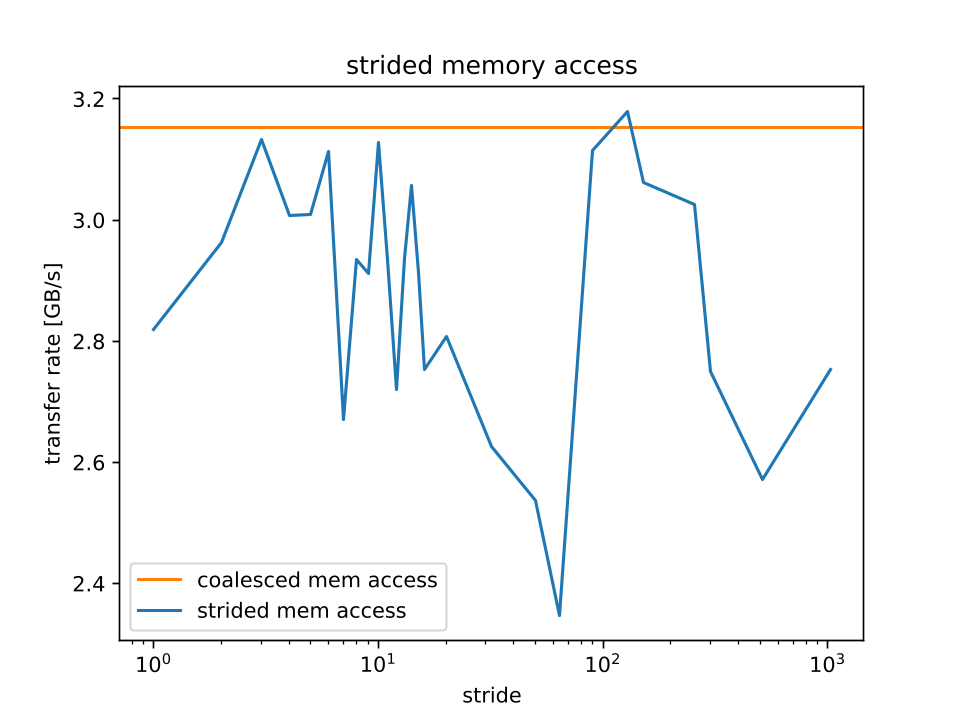
\includegraphics[scale=0.7]{pictures/strided_thread_access.png}
    \caption{exercise 3.3, thread access with stride}
    \label{fig:2.3}
\end{figure}